\chapter{Experimental Setup}
\label{ch:exp}

All data analysed in this thesis was recorded with the CMS experiment at the Large Hadron
Collider (LHC) at the European Organization for Nuclear Research (CERN) near Geneva, Switzerland.
This chapter provides a short overview of CERN and its accelerators, the LHC, as well as a
short description of the main components of the CMS experiment.

\section{The Large Hadron Collider}
\label{sec:lhc}
The LHC \cite{lhc_designreport} is currently by far the largest and most powerful particle accelerator in
the world. It is a circular accelerator situated in a tunnel around 100 metres below the Swiss-French
border west of Geneva. Its main purpose is accelerating protons to energies of up to 13 TeV
\footnote{One electronvolt (TeV) is the energy acquired by a charge of 1$e$ passing through an electron field of 1 volt, equivalent to \num{1.602e-19} Joule.} 
in the final development stage of the machine starting in 2015. 
Besides the acceleration of protons it is also capable of accelerating heavy ions (predominantly lead ions) to energies of up to 
2.76 TeV per nucleon.

\subsection{The acceleration chain}
\label{sub:chain}
Particles injected into the LHC for final acceleration are required to have an energy of 450 GeV. This is
achieved by a long chain of linear and circular accelerators, a sketch of which can be seen in
Fig.~\ref{fig:accelerators}. 

\begin{figure}[h!]
    \label{fig:accelerators}
    \caption{Conceptual drawing of all accelerators and experiments hosted at CERN. Besides operating
    the LHC, there are many other accelerators, decelerators and experiments being operated.}
    \centering
    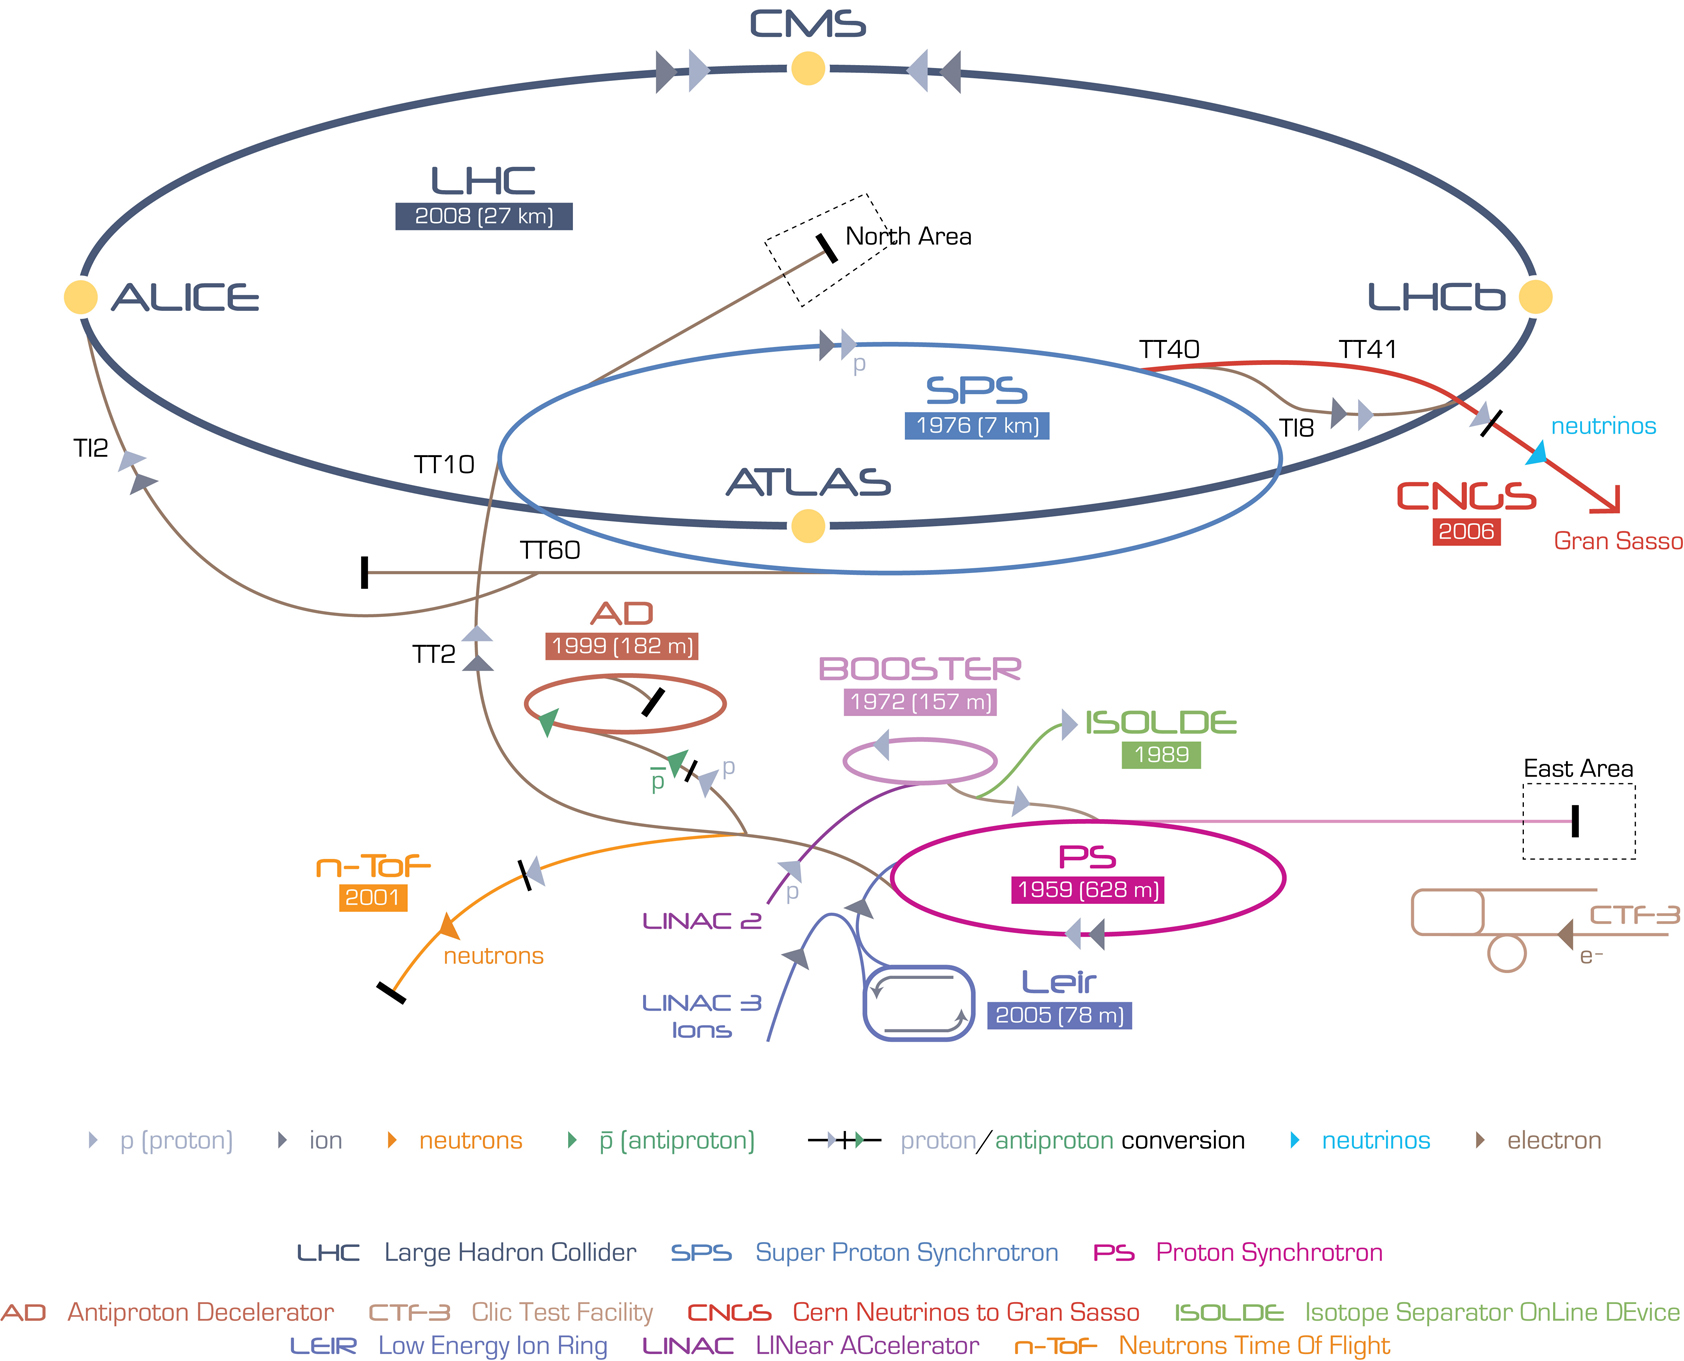
\includegraphics[width=0.65\textwidth]{../figs/Cern-Accelerator-Complex.jpg}
\end{figure}

Protons used for acceleration in the LHC are extracted from a hydrogen molecules in a bottle situated 
at the CERN main site. These molecules are stripped of their electrons by strong electric fields
and subsequently injected into the first acceleration stage, the linear accelerator Linac 2. Upon exiting
Linac 2, the protons have gained an energy of 50 MeV and are injected into the first circular accelerator,
the Booster. This synchrotron with a circumference of 157 meters accelerates the protons to an energy of 1.4 GeV and
uses magnetic dipole fields to bend the protons onto a circular path. These bending magnets are operated at 
room temperature for the Booster and in fact all the accelerators up to the LHC.
From the Booster, the protons are injected further into the Proton Synchrotron, an accelerator originally built
in 1959 with a circumference of 628 meters and an output energy of 25 GeV. The last step before injection into
the LHC is the Super Proton Synchrotron (SPS), which accelerates the protons to the LHC injection energy of 450 GeV.
The SPS is the world's second largest accelerator with a circumference of nearly 7 km, and it was the first accelerator
to collide protons and anti-protons at energies high enough to produce $W$ and $Z$ bosons, leading to their discovery in 1983
\cite{Wdiscovery, Zdiscovery}.

Ions pass through the same accelerators on their way to the LHC, the only difference being the
first linear accelerator, which in the case of heavy ions is Linac 3.

While the LHC is filled and delivering collisions to its experiments, the accelerators are used to provide high
energy particles to other experiments ongoing at CERN. The 
